\documentclass{article}

\usepackage{amsfonts,relsize,amsmath,amssymb,systeme}
\usepackage{listings}

\usepackage{hyperref}

\usepackage{graphicx}
\graphicspath{ {./images/} }

\usepackage[T1]{fontenc}
\usepackage[polish]{babel}
\usepackage[utf8]{inputenc}
\usepackage{lmodern}
\selectlanguage{polish}
\author{Autor: Zbigniew Królikowski
\\\\\\\\}
\title{ Algorytmy dla Problemów Trudnych Obliczeniowo.\\
Rozwiązanie zadania: \textbf{Potęga hetmanów}
Informatyka 2015/16}


\begin{document}
\maketitle


\vfill

\paragraph{Prowadzący: dr hab. inż. Piotr Faliszewski
\\\\\\\\
}

\newpage

\section{Uwagi}

Moja filozofia zapisu: \textbf{hetmany bijące nie zmieniają miejsca tylko znikają na rzecz zbitego} - taki obraz przyjąłem gdyż łatwiej było go rozpisać, mniej dynamiki. Często zapisuję bicie jako redukcję. Nie zmienia to w żaden sposób istoty algorytmu tylko jego opis, który mógłby być mylący bez tej notki.

\section{Reprezentacja problemu}

Plansza została przedstawiona jako \textbf{graf nieskierowany}, w którym każdy węzeł połączony jest z innymi co najwyżej 8 krawędziami.

\subsection{Zapis wartości hetmanów}

W celach uproszczenia obliczeń wartości są reprezentowane jako wykładniki liczby 2.

\subsection{Krótki słownik moich pojęć - w razie wątpliwości}

\begin{itemize}
\item osie - pion, poziom i skosy
\end{itemize}

\clearpage

\section{Wstępne obserwacje}

\section{Ogranicznie maksymalnej wartości hetmana}

Na wartość końcową hetmana da się nałożyć pewne ograniczenie:

\textbf{Końcowa wartość hetmana $h$ nie może być wyższa od jego aktualnej wartości $V(h) * 2^n$ gdzie $n$ - liczba hetmanów w pionie, poziomie i na skosach (osiach).}

Jest to łatwo udowodnić - każde bicie skierowane przeciwko hetmanowi podnosi jego wartość dwukrotnie. Bić może być \textit{w najlepszym wypadku} tyle ile hetmanów będących na tych samych osiach co dany hetman.

\begin{figure}[!ht]
  \centering
      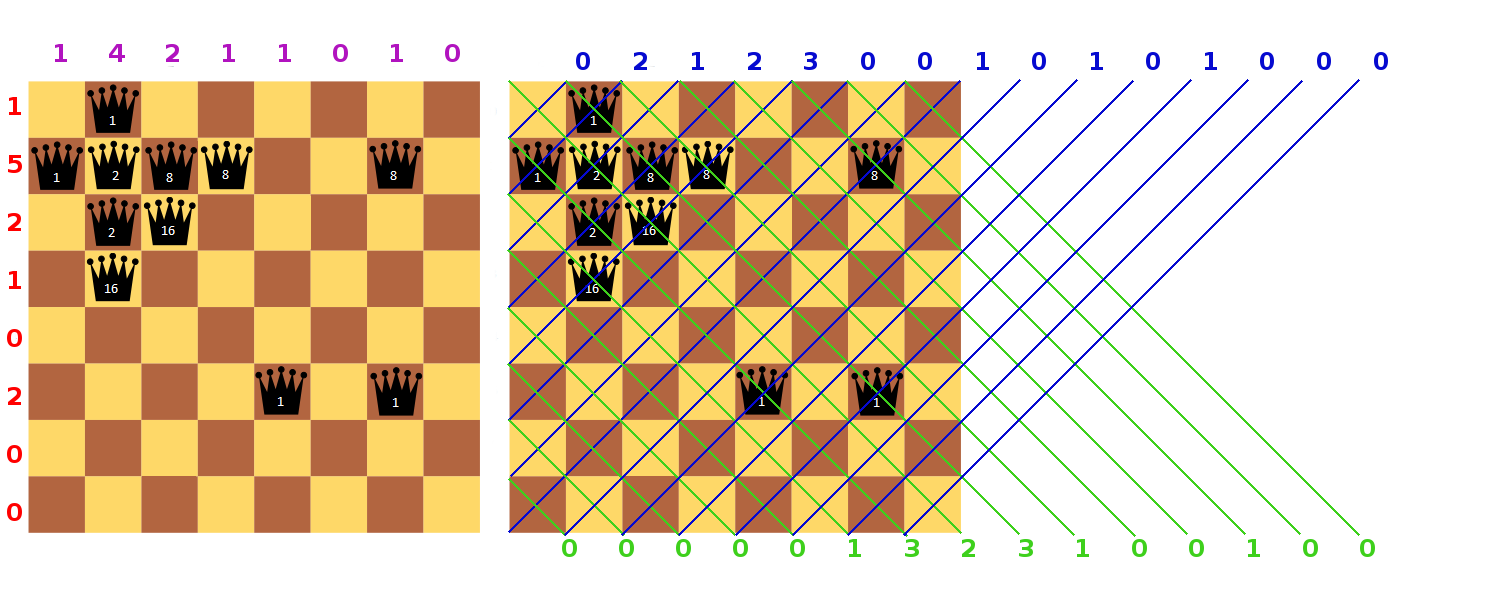
\includegraphics[scale=0.3]{obs1.png}
  \caption{Zliczenie ilości hetmanów na poszczególnych osiach.}
\end{figure}

\clearpage 

\begin{figure}[!ht]
  \centering
      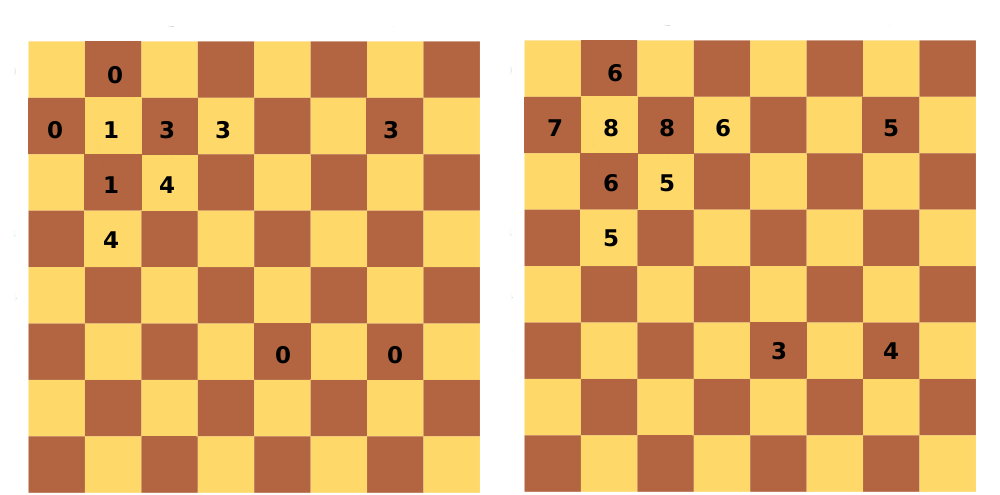
\includegraphics[scale=0.25]{obs1a.png}
  \caption{\textit{Lewo:} Wartość hetmanów w mojej notacji \textit{Prawo:} maksymalna ilość bić skierowana ku konkretnemu hetmanowi.\textit{ Dół:} Górne ograniczenie na wartość końcową hetmanów. Na czerwono hetmany, które nie mogą być końcowe dla K=1.}
  
\end{figure}

Jak zademonstrowano na powyższym przykładzie możemy \textbf{wykluczyć} pewne kombinacje(o wielkości K) hetmanów z bycia końcowymi. Warunkiem wykluczenia jest niemożliwość uzyskania przez tą kombinację wartości będącej sumą wartości wszystkich hetmanów na planszy. Jest to pewne uproszczenie problemu, część postaci rozwiązania.

\paragraph{Bezpośrednio nieużyteczne -}liczba tych kombinacji wynosi $\binom{N} {K}$ gdzie $N$ to liczba hetmanów na planszy a $K$ to ilość hetmanów końcowych.

\subsubsection{Heurystyka}

Możemy się zatem spodziewać, że pewne hetmany zostaną zredukowane "wcześniej niż później", a więc mamy nałożoną jakąś \textbf{kolejność przeszukiwania} przestrzeni rozwiązań. \textbf{Skoro mniejszy potencjał hetmana wiąże się z niemożnością bycia końcowym hetmanem to może powinniśmy ruszać się  wcześniej tymi z mniejszym potencjałem?}

\section{Algorytm}

Algorytm przeszukuje przestrzeń rozwiązań za pomocą wywołań rekurencyjnych modyfikując za każdym razem planszę. Kolejność przeszukiwania jest heurystyką, która zostanie później opisana.

\begin{lstlisting}
bool recursiveCheck():
	if achievedTarget():
		return true
	else:
		sortQueens()
		for queen in board:
			connections = queen.possibleConnections()
			sortConnections()
			for connection in connections:
				move(connection)
				if recursiveCheck():
					return true
	// Nie znaleziono rozwiazania	
		undoMove()	
		return false
		
bool achievedTarget():
	return currentQueens <= targetQueens
\end{lstlisting}

\subsection{SortConnections}

Zadaniem tego algorytmu jest porządkowanie połączeń wychodzących z danego hetmana. W końcowej wersji nie nałożyłem tutaj żadnego heurystycznego porządku - wszystkie testowane heurystyki okazały się nieużyteczne.

\section{Generator scenariuszy}

Dodatkowo wykonałem w języku Python generator który dla danej wielkości planszy, końcowej ilość hetmanów i docelowej ilości ruchów tworzy losowy scenariusz wraz z przykładowym rozwiązaniem.

Okazał się on bardzo przydatny w testowaniu algorytmu.


\end{document}
